\documentclass{beamer}
\usetheme{Singapore}
\usepackage{changepage}

%\usepackage{pstricks,pst-node,pst-tree}
\usepackage{amssymb,latexsym}
\usepackage{tikz}
\usepackage{graphicx}
\usepackage{fancyvrb}
\usepackage{hyperref}
\usepackage{fancybox}
\usepackage[listings]{tcolorbox}

\definecolor{codegreen}{rgb}{0,0.6,0}
\definecolor{codegray}{rgb}{0.5,0.5,0.5}
\definecolor{codepurple}{rgb}{0.58,0,0.82}
\definecolor{backcolour}{rgb}{0.95,0.95,0.92}

\lstdefinestyle{mystyle}{
    language=Python,
    backgroundcolor=\color{backcolour},   
    commentstyle=\color{codegreen},
    keywordstyle=\color{magenta},
    numberstyle=\tiny\color{codegray},
    stringstyle=\color{codepurple},
    basicstyle=\ttfamily\footnotesize,
    breakatwhitespace=false,         
    breaklines=true,                 
    captionpos=b,                    
    keepspaces=true,                 
    numbers=left,                    
    numbersep=5pt,                  
    showspaces=false,                
    showstringspaces=false,
    showtabs=false,                  
    tabsize=2,
    escapechar=|,
    frame=single
}

\lstset{style=mystyle}


\newcommand{\bi}{\begin{itemize}}
\newcommand{\li}{\item}
\newcommand{\ei}{\end{itemize}}
\newcommand{\Show}[1]{
\begin{center}
\shadowbox{\begin{minipage}{0.8\textwidth}
          #1
          \end{minipage}}
\end{center}
}
\newcommand{\arrow}{\ensuremath{\rightarrow}}

\newcommand{\uparr}{\ensuremath{\uparrow}}


\newcommand{\fig}[2]{\centerline{\includegraphics[width=#1\textwidth]{#2}}}

\newcommand{\bfr}[1]{\begin{frame}[fragile]\frametitle{{ #1 }}}
\newcommand{\efr}{\end{frame}}

\newcommand{\cola}{\begin{columns}\begin{column}{0.5\textwidth}}
\newcommand{\colb}{\end{column}\begin{column}{0.5\textwidth}}
\newcommand{\colc}{\end{column}\end{columns}}


\title{Think Python 2e, Chapter 18 Notes}
\author{Inheritance}

\begin{document}

\begin{frame}
\maketitle
\end{frame}

\bfr{Card objects}

\cola
Encoding of suits:\\

\begin{tabular}{rcl}
Spades & $\rightarrow$ & 3\\
Hearts & $\rightarrow$ & 2\\
Diamonds & $\rightarrow$ & 1\\
Clubs & $\rightarrow$ & 0\\
\end{tabular}
\colb
Encoding of ranks:\\

\begin{tabular}{rcl}
Ace & $\rightarrow$ & 1\\
...\\
Jack & $\rightarrow$ & 11\\
Queen & $\rightarrow$ & 12\\
King & $\rightarrow$ & 13\\
\end{tabular}
\colc

\end{frame}

\bfr{Class definition of card:}
\begin{lstlisting}
class Card:
    """Represents a standard playing card."""

    def __init__(self, suit=0, rank=2):
        self.suit = suit
        self.rank = rank
\end{lstlisting}
\begin{lstlisting}
queen_of_diamonds = Card(1, 12)
\end{lstlisting}

\end{frame}

\bfr{Class attributes}
\begin{lstlisting}
# inside class Card:

suit_names = ['Clubs', 'Diamonds', 'Hearts', 'Spades']
rank_names = [None, 'Ace', '2', '3', '4', 
              '5', '6', '7', '8', '9', '10',
              'Jack', 'Queen', 'King']

def __str__(self):
    return '%s of %s' % (Card.rank_names[self.rank],
                         Card.suit_names[self.suit])

\end{lstlisting}
\bi
\li Variables declared inside a class but outside of any
method, like \lstinline{suit_names} and \lstinline{rank_names}
 are {\bf class variables}.
\li They are associated with the class \lstinline{Card}
\li Variables like \lstinline{suit} and \lstinline{rank} are 
{\bf instance variables}
\ei

\end{frame}


\bfr{Creating cards}
\begin{lstlisting}
>>> card1 = Card(1, 11)
>>> print(card1)
Jack of Diamonds
\end{lstlisting}

\includegraphics{statediagram18-1}

\end{frame}


\bfr{Comparing cards}
\begin{lstlisting}
# inside class Card:

    def __lt__(self, other):
        # check the suits
        if self.suit < other.suit: return True
        if self.suit > other.suit: return False

        # suits are the same... check ranks
        return self.rank < other.rank
\end{lstlisting}
More succinctly:
\begin{lstlisting}
# inside class Card:

    def __lt__(self, other):
        t1 = self.suit, self.rank
        t2 = other.suit, other.rank
        return t1 < t2
\end{lstlisting}


\end{frame}
\bfr{Decks}
\begin{lstlisting}
class Deck:

    def __init__(self):
        self.cards = []
        for suit in range(4):
            for rank in range(1, 14):
                card = Card(suit, rank)
                self.cards.append(card)
\end{lstlisting}


\end{frame}

\bfr{Printing a deck}
\begin{lstlisting}
# inside class Deck:

    def __str__(self):
        res = []
        for card in self.cards:
            res.append(str(card))
        return '\n'.join(res)
\end{lstlisting}

\begin{lstlisting}
>>> deck = Deck()
>>> print(deck)
Ace of Clubs
2 of Clubs
3 of Clubs
...
10 of Spades
Jack of Spades
Queen of Spades
King of Spades
\end{lstlisting}


\end{frame}

\bfr{Add, remove, and shuffle cards}
\begin{lstlisting}
# inside class Deck:

    def pop_card(self):
        return self.cards.pop()

    def add_card(self, card):
        self.cards.append(card)       
     
    def shuffle(self):
        random.shuffle(self.cards)
\end{lstlisting}

\bi
\li
A method like these that doesn't do much is called a {\bf veneer}.
\li
It improves the interface of the implementation.
\ei

\end{frame}

\bfr{Inheritance}
\begin{lstlisting}
class Hand(Deck):
    """Represents a hand of playing cards."""

    def __init__(self, label=''):
        self.cards = []
        self.label = label
\end{lstlisting}

\bi
\li
\lstinline{Hand} {\bf inherits} all attributes and methods from \lstinline{Deck}.
\li
\lstinline{Deck} is the {\bf parent} and \lstinline{Hand} is the {\bf child}.

\ei

\end{frame}
\bfr{Inheritance}
\begin{lstlisting}
class Hand(Deck):
    def __init__(self, label=''):
        self.cards = []
        self.label = label
\end{lstlisting}
\begin{lstlisting}
>>> hand = Hand('new hand')
>>> hand.cards
[]
>>> hand.label
'new hand'
>>> deck = Deck()
>>> card = deck.pop_card()
>>> hand.add_card(card)
>>> print(hand)
King of Spades
\end{lstlisting}
\bi
\li \lstinline{__str__} and \lstinline{add_card} don't have to be defined
for \lstinline{Hand}
\ei


\end{frame}



\bfr{Inheritance}
\begin{lstlisting}
# inside class Deck:

    def move_cards(self, hand, num):
        for i in range(num):
            hand.add_card(self.pop_card())
\end{lstlisting}
\end{frame}

\bfr{Inheritance}
\bi

\li We can now move cards from the deck to  a hand, from a hand to a hand,
from a hand to the deck, {\em etc.}
\li
Inheritance can facilitate code reuse.
\li Inheritance sometimes mimics the natural structure of a problem.
\li Inheritance can make it difficult to debug.
\ei
\begin{center}
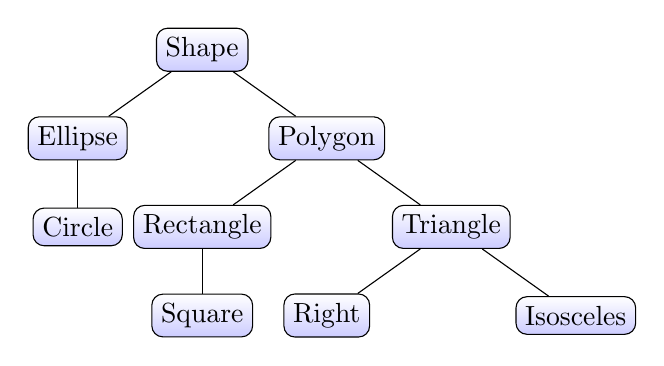
\begin{tikzpicture}[sibling distance=12em, scale=0.75,
  every node/.style = {shape=rectangle, rounded corners,
    draw, align=center,
    top color=white, bottom color=blue!20}]]
  \node {Shape}
    child { node {Ellipse} child { node {Circle} }}
    child { node {Polygon}
      child { node {Rectangle}
        child { node {Square} }}
      child { node {Triangle}
        child { node {Right} }
        child { node {Isosceles} }}
};

\end{tikzpicture}
\end{center}

\end{frame}

\bfr{Class diagrams}
\centerline{\includegraphics{classdiagram18-2}}

Class relationships:
\bi
\li A deck {\bf HAS-A} card
\bi \li the * shows {\bf multiplicity}\ei
\li A hand {\bf IS-A} deck
\li A class required by another class for other reasons is a {\bf dependency}
\bi
\li {\em e.g.} used as parameters or for internal computation 
\li shown with dotted lines \ei
\ei


\end{frame}

\bfr{Debugging}
\bi

\li Inheritance can make it hard to find which method is invoked.
\li Can use this function:
\begin{lstlisting}
def find_defining_class(obj, meth_name):
    for ty in type(obj).mro():
        if meth_name in ty.__dict__:
            return ty
\end{lstlisting}
\begin{lstlisting}
>>> hand = Hand()
>>> find_defining_class(hand, 'shuffle')
<class '__main__.Deck'>
\end{lstlisting}

\li \lstinline{mro} stands for "method resolution order"

\ei

\end{frame}

\bfr{Liskov substitution principle}
\bi
\li When you override a method:
\bi
\li new method should be same as old method
\li take same parameters
\li return same type
\li obey same preconditions
\li obey same postconditions
\ei
\li Any function designed to work with a parent class
will also work with a child class.
\ei

\end{frame}

\bfr{Data encapsulation}

\bi
\li In the \lstinline{markov} function from chapter 13 we used
two global variables:
\bi 
\li
\lstinline{suffix_map = dict()}
\li
\lstinline{prefix = ()}
\ei
\li If we wanted to read two texts in the same program
their prefixes and suffixes would get mixed up.
\li Encapsulate each with an object:
\begin{lstlisting}
class Markov:

    def __init__(self):
        self.suffix_map = dict()
        self.prefix = ()    
\end{lstlisting}
\ei


\end{frame}


\bfr{Data encapsulation}

\bi
\li We now translate functions with global variables into methods:
\ei
\begin{lstlisting}
def process_word(self, word, order=2):
    if len(self.prefix) < order:
        self.prefix += (word,)
        return

    try:
        self.suffix_map[self.prefix].append(word)
    except KeyError:
        # if no entry for this prefix, make one
        self.suffix_map[self.prefix] = [word]

    self.prefix = shift(self.prefix, word)        
\end{lstlisting}
\bi
\li An important example of {\bf refactoring}
\ei


\end{frame}

\bfr{Object oriented development}
\bi
\li Start with global variables when necessary
\li Finish working program
\li Look for associations between global variables
\li Encapsulate related variables as attributes
\li Transform associated functions into methods
\li We will do this wiht the Mandelbrot program!
\ei

\end{frame}

\bfr{Vocabulary}
\begin{description}

\li[encode:]
To represent one set of values using another set of values by constructing a mapping between them.
\li[class attribute:]
An attribute associated with a class object. Class attributes are defined inside a class definition but outside any method.
\li[instance attribute:]
An attribute associated with an instance of a class.
\li[veneer:]
A method or function that provides a different interface to another function without doing much computation.
\end{description}
\end{frame}
\bfr{Vocabulary}
\begin{description}
\li[inheritance:]
The ability to define a new class that is a modified version of a previously defined class.
\li[parent class:]
The class from which a child class inherits.
\li[child class:]
A new class created by inheriting from an existing class; also called a “subclass”.
\end{description}
\end{frame}
\bfr{Vocabulary}
\begin{description}
\li[IS-A relationship:]
A relationship between a child class and its parent class.
\li[HAS-A relationship:]
A relationship between two classes where instances of one class contain references to instances of the other.
\li[dependency:]
A relationship between two classes where instances of one class use instances of the other class, but do not store them as attributes.
\end{description}
\end{frame}
\bfr{Vocabulary}
\begin{description}
\li[class diagram:]
A diagram that shows the classes in a program and the relationships between them.
\li[multiplicity:]
A notation in a class diagram that shows, for a HAS-A relationship, how many references there are to instances of another class.
\end{description}
\end{frame}
\bfr{Vocabulary}
\begin{description}
\li[data encapsulation:]
A program development plan that involves a prototype using global variables and a final version that makes the global variables into instance attributes.
\end{description}
\end{frame}

\end{document}
